\documentclass[12pt,letter]{article}

% Core packages
\usepackage{geometry}
\geometry{margin=2cm}
\usepackage{amsmath,amsfonts,amssymb}
\usepackage{graphicx}
\usepackage{enumitem}
\usepackage{hyperref}
\usepackage{setspace}
\usepackage{xcolor}
\usepackage{float}
\usepackage{algorithm}
\usepackage{algpseudocode}
\usepackage{fancyhdr}
\usepackage{fontspec} 
\usepackage{textcomp} 
\usepackage{caption}
\usepackage{fancyvrb}
\usepackage{tikz}
\usepackage{ragged2e}
\usepackage[patch=none]{microtype}
\usepackage{xstring}
\usepackage{multirow}
\usepackage{pdfpages}
\usepackage{adjustbox}
\usetikzlibrary{arrows.meta, shapes.geometric, arrows, positioning, fit, calc}

% Font setup
\setmainfont{Noto Sans}[
Weight=Regular,
Scale=1.0
]
\setmonofont{Space Mono}[Scale=0.9]

\usepackage{fvextra} % Enhanced version of fancyvrb
\usepackage{listings}
% Define Rust language style for listings
\lstdefinestyle{rust}{
basicstyle=\ttfamily\small,
frame=single,
breaklines=true,
showstringspaces=false,
showspaces=false,
columns=fullflexible,
keepspaces=true,
alsoletter={\_},
escapeinside={(*@}{@*)},
mathescape=false,
texcl=false,
upquote=true,
morecomment=[l]{;},
morecomment=[l]{//},
morecomment=[l]{///},
escapechar=¡,
tabsize=3
}
\renewcommand{\refname}{REFERENCES}
\hyphenpenalty=10000
\exhyphenpenalty=10000
\setlength{\parskip}{0.25cm}
\newcommand{\patentfigure}[2]{%
  \begin{figure}[htbp]
    \centering
    #1
    \caption{#2}
    \label{fig:\thefigcounter}
  \end{figure}
  \stepcounter{figcounter}%  % This line increments the counter
}

\renewcommand{\lstlistingname}{Figure}
% Define common verbatim environment options
\fvset{
frame=single,
fontsize=\small,
commandchars=\\\{\},
formatcom=\color{black}
}
\renewcommand{\thefigure}{\thefigcounter}
\newcounter{paracounter}
\setcounter{paracounter}{1}
\newcommand{\ppara}[1]{
\noindent\textbf{[\formatparanumber{\arabic{paracounter}}]} \begingroup\RaggedRight\sloppy\hbadness=10000 #1\par\endgroup%
\stepcounter{paracounter}%
}
\newcommand{\formatparanumber}[1]{%
\ifnum#1<10 000%
\else\ifnum#1<100 00%
\else\ifnum#1<1000 0%
\fi\fi\fi#1%
}

\newcounter{figcounter}
\setcounter{figcounter}{1}

% For section numbering
\renewcommand{\thesection}{Arabic{section}}
\renewcommand{\thesubsection}{\thesection.\arabic{subsection}}

% Line spacing
\onehalfspacing

% Page headers/footers
\pagestyle{fancy}
\fancyhf{}
\fancyhead[R]{TWO'S COMPLEMENT FLOATING POINT ARITHMETIC SYSTEM}
\fancyfoot[C]{Page \thepage}
\renewcommand{\headrulewidth}{0.4pt}
% Set the entire document to ragged right alignment with no warnings
\RaggedRight
\sloppy
\hbadness=10000
\tolerance=10000
\emergencystretch=3em

\title{\textbf{TWO'S COMPLEMENT FLOATING POINT ARITHMETIC SYSTEM}}
\author{Nick Spiker}
\date{\today}

\begin{document}

% Beginning of document
\begin{titlepage}
\begin{center}
\vspace*{1cm}
{\huge \textbf{TWO'S COMPLEMENT FLOATING POINT}\par}
{\huge \textbf{ARITHMETIC SYSTEM}\par}
\vspace{2cm}
{\Large Provisional Patent Application\par}
\vspace{2.5cm}
{\Large Inventor: Nick Spiker\par}
\vspace{1cm}
{\Large \today\par}
\end{center}
\end{titlepage}

\newpage
% Make sections appear in the table of contents
\renewcommand{\contentsname}{TABLE OF CONTENTS}
\makeatletter
\let\stdl@section\l@section
\renewcommand{\l@section}[2]{%
  \stdl@section{\textbf{#1}}{\textbf{#2}}%
}
\makeatother

% Add starred sections to TOC manually
\addcontentsline{toc}{section}{ABSTRACT}
\addcontentsline{toc}{section}{TECHNICAL FIELD}
\addcontentsline{toc}{section}{BACKGROUND}
\addcontentsline{toc}{section}{SUMMARY OF THE INVENTION}
\addcontentsline{toc}{section}{LIST OF FIGURES}
\addcontentsline{toc}{section}{DETAILED DESCRIPTION}
\addcontentsline{toc}{section}{ECONOMIC ADVANTAGES}
\addcontentsline{toc}{section}{IMPLEMENTATION CONSIDERATIONS AND CONCLUSION}
\addcontentsline{toc}{section}{CLAIMS}
\addcontentsline{toc}{section}{REFERENCES}

\tableofcontents
\newpage
%==============================================================================
% Abstract
%==============================================================================
\section*{ABSTRACT}

The SPIRIX system introduces a fundamentally new approach to floating-point arithmetic by employing two's complement representation thruout the calculation pipeline without a separate sign bit. Unlike IEEE-754's sign-magnitude approach, SPIRIX uses left-aligned normalized fractions and unbiased exponents to represent both real (Scalar) and complex (Circle) numbers within a continuous mathematical framework.

A key innovation is SPIRIX's consistent handling of mathematical infinities following Riemann principles, maintaining identities such as: non-zero divided by zero produces infinity; infinity times any non-zero value returns infinity; zero divided by any non-zero value remains zero; and products involving zero remain zero unless indeterminate. For values beyond normal representation, SPIRIX introduces "exploded" (exceeding maximum magnitude) and "vanished" (below minimum magnitude) states that preserve phase information, enabling mathematical consistency even at the extremes. This maintains critical properties that can be compromised in IEEE-754: operations like squaring the maximum representable value properly yield infinity, multiplication of two non-zero non-infinite values never produces infinity, and multiplication of two non-zero values never results in zero. These mathematical consistencies eliminate numerous edge cases that typically require special handling in floating-point implementations.

The system identifies the specific cause of ambiguous operations thru distinct bit patterns in the fraction component while using a single reserved exponent value, enabling precise error tracing without extensive conditional testing. The system's parameterized design allows independent selection of fraction and exponent sizes, enabling applications to optimize precision and range according to specific requirements. By maintaining two's complement properties thruout, SPIRIX achieves subtractive equivalence (a-b=0 if and only if a=b) and multiplicative reciprocal coherence without special-case handling, addressing longstanding limitations in floating-point arithmetic while providing a mathematically consistent framework suitable for modern computing environments.

%==============================================================================
% Technical Field
%==============================================================================
\section*{TECHNICAL FIELD}

\ppara{The present invention relates to computer arithmetic operations, and more particularly to a system and method for implementing floating-point arithmetic operations using two's complement representation thruout the entire calculation pipeline. This invention outlines a comprehensive approach to handling numerical values outside standard representation ranges, preserving operation cause in undefined operations, and providing a unified framework for both real and complex number arithmetic in computing systems. The invention improves mathematical consistency by ensuring multiplication and division operations preserve non-zero status, maintaining subtractive identities without requiring subnormal numbers, and establishing well-defined arithmetic behaviors for singularities like zero and infinity. The invention has applications in digital signal processing, scientific computing, machine learning, graphics rendering, financial modeling, and any computational domain requiring high-performance floating-point arithmetic with configurable precision and range characteristics where mathematical consistency is paramount.}

%==============================================================================
% Background
%==============================================================================
\section*{BACKGROUND}

\ppara{Floating-point arithmetic is a fundamental component of modern computing systems, providing a means to represent and manipulate numbers within digital hardware constraints. Since 1985, the IEEE-754 standard has been the predominant specification for floating-point computation, defining formats for representing floating-point numbers and protocols for arithmetic operations.}

\ppara{The IEEE-754 standard employs a structure where floating-point numbers are represented using three distinct components: a sign bit, an exponent, and a mantissa (also known as the significand). This representation requires specialized hardware or software implementations to handle the sign bit separately from the magnitude components, leading to complicated testing and branching for most operations.}

\ppara{Despite its widespread adoption, the IEEE-754 standard has several key limitations:}

\ppara{First, it requires extensive special case handling for operations involving special values like NaN (Not a Number), infinities, zeros, and subnormal numbers, greatly increasing implementation complexity. The separate sign bit creates additional logic for operations, as adding two negatives utilizes addition logic with sign adjustment while adding opposite signs uses separate subtraction logic with potential zero crossing and possible sign adjustment. When an operation produces a NaN, information about what caused the invalid operation is lost, complicating debugging and error tracing. The many special cases and state testing required for IEEE-754 operations creates performance bottlenecks, especially in SIMD operations. Furthermore, IEEE-754 violates important mathematical properties, such as allowing the product of non-zero values to equal zero when the result underflows, and requiring subnormal numbers to maintain the property that x = y if and only if x - y = 0. Finally, the fixed allocation of bits between the exponent and mantissa in IEEE-754 formats like binary32 and binary64 lack the flexibility needed for many applications.}

\ppara{Several alternative approaches to floating-point representation have attempted to address IEEE-754's limitations with varying success. Logarithmic number systems (LNS) represent numbers as logarithms, simplifying multiplication and division but greatly complicating addition and subtraction. Posit number systems employ a tapered precision approach with a variable-length exponent field that automatically adjusts based on magnitude, but they still use sign-magnitude representation rather than two's complement thruout. Other alternatives include fixed-point arithmetic (integer/constant), Unums (Universal Numbers), dual floating-point approaches, and decimal floating-point standards, but these solutions add complexity without resolving the fundamental architectural challenges inherent in sign-magnitude representations.}

\ppara{While these alternative approaches address certain aspects of IEEE-754's limitations, none provide a comprehensive solution that improves both mathematical consistency and computational efficiency across the full spectrum of numerical operations. Furthermore, no existing system incorporates: complete elimination of the separate sign bit in favor of two's complement representation; systematic tracking of phase and orientation information for values exceeding normal representation ranges; a comprehensive scheme for identifying and preserving the cause of undefined operations; a unified approach to both real and complex number representation with shared exponent; guaranteed non-zero results when multiplying or dividing non-zero values; and independent selection of fraction and exponent sizes allowing applications to optimize for either precision or range according to their requirements.}

\ppara{There is, therefore, a need for an improved approach to floating-point arithmetic that addresses these limitations while maintaining or improving computational accuracy and efficiency.}

%==============================================================================
% Summary of the Invention
%==============================================================================
\section*{SUMMARY OF THE INVENTION}

\ppara{The present invention provides a novel floating-point arithmetic system that uses two's complement representation thruout the full calculation pipeline. This approach fundamentally reimagines how numerical values are represented and manipulated in computing systems, offering significant advantages over traditional IEEE-754 and other floating point implementations.}

\ppara{At its core, the system represents numbers using two primary components: a normalized two's complement fraction and an unbiased two's compliment exponent. Unlike IEEE-754, which uses a separate sign bit, magnitude representation and biased exponent, this system leverages the natural properties of two's complement arithmetic to simplify operations while expanding the capabilities of floating-point computations. This allows for "escaped" values, where values "vanish" [$\downarrow$] when they go below the range of representable magnitude or "explode" [$\uparrow$] when they exceed the maximum exponent value. These escaped states maintain their phase information, preserving mathematical continuity—for example, a negative vanished value multiplied by a negative vanished value returns a positive vanished value.}

\ppara{Key innovations of the system include:}

\ppara{Unified representation for both real (Scalar) and complex (Circle) values, with consistent operation semantics across both domains.}

\ppara{Preservation of operation cause in undefined states, providing error tracking and debugging compared to IEEE-754's single ambiguous NaN value.}

\ppara{Consistent handling of numerical states thru normalization levels, with explicit tracking of values that have "escaped" normal representation due to being too large (exploded) or too small (vanished).}

\ppara{Independent selection of fraction and exponent sizes, allowing applications to optimize for their specific range and precision requirements.}

\ppara{Native support for complex arithmetic operations without requiring separate real and imaginary component handling.}

\ppara{Simplified hardware implementation thru consistent use of two's complement arithmetic thruout the pipeline, eliminating the need for separate sign bit logic and subsequent case handling.}

\ppara{The system introduces a normalization scheme with multiple levels to represent different numeric states, wherein fractions are left-aligned. Normal numbers utilize N-1 normalization to retain sign information. Exploded values, vanished values, and various undefined states each have their designated normalization levels, enabling tracking of numerical state thruout calculations. A single reserved exponent value (one followed by all zeros, designated as AMBIGUOUS\_EXPONENT) is utilized for all ambiguous cases, thereby enabling efficient checking prior to performing operations.}

\ppara{In the system, complex values are represented as "Circles," wherein both real and imaginary components share the same exponent, maintaining binary fraction alignment and thereby greatly simplifying checks and calculations. This unified approach enables branchless hardware implementation of normal complex operations without requiring separate handling mechanisms for real and imaginary components.}

\ppara{The invention includes specific implementations for all fundamental arithmetic operations (addition, subtraction, multiplication, division), transcendental functions, and bit manipulation operations, maintaining mathematical consistency below, within, and beyond the exponent range of representable values. Particular attention is given to boundary conditions and transitions between different states to ensure that operations remain reliable when values exceed representable magnitude or become undefined. The system architecture allows for future enhancement and versioning as the format evolves.}

\ppara{By eliminating the requirement for sign bit branches and providing a unified approach to both real and complex arithmetic, the invention offers a more elegant and efficient solution for numerical computation, particularly in domains requiring configurable precision, fast and uniform computation (SIMD) or extensive use of complex numbers such as Fast Fourier Transforms (FFT).}

\section*{DEFINITIONS}

\ppara{As used herein, the following terms shall have the following meanings, unless the context clearly indicates otherwise:}

\ppara{\textbf{"Two's complement representation"} refers to a method of representing positive and negative integers where the most significant bit (leftmost) can be checked to determine the sign (0 for positive, 1 for negative). Negative values are encoded by taking the bit complement (logical NOT) of the absolute value and adding one. In this invention, two's complement representation is applied to floating-point components thruout the entire calculation pipeline, eliminating the need for separate sign bit handling for all basic operations (add, subtract, multiply, divide).}

\ppara{\textbf{"Scalar"} refers to a data type representing real numbers using two primary components: a normalized two's complement fraction and an unbiased two's compliment exponent. Unlike traditional floating-point formats with separate sign bit, the Scalar's sign information is naturally encoded within the fractions two's complement representation.}

\ppara{\textbf{"Circle"} refers to a data type representing complex numbers using three components: a real fraction, an imaginary fraction, and a shared exponent (all in two's complement representation). The shared exponent ensures that both components maintain relative magnitudes, simplifying complex arithmetic operations.}

\ppara{\textbf{"Fraction"} refers to the component of a Scalar or Circle that stores the normalized significand in two's complement format. The size of the fraction determines the precision of the representation, and its most significant bits encode state information thru normalization levels. Fraction sizes are denoted in shorthand powers of two for convenience and indicated as F3, F4, F5, F6, or F7, corresponding to 8-bit (2³), 16-bit (2⁴), 32-bit (2⁵), 64-bit (2⁶), and 128-bit (2⁷) integer representations respectively. For example, an F5 fraction uses a 32-bit (2⁵) integer to store the significand, providing approximately 9.4 decimal digits of precision.}

\ppara{\textbf{"Exponent"} refers to the component of a Scalar or Circle that determines the scale of the value. The size of the exponent determines the representable range. Unlike traditional floating-point formats that use biased exponents, this invention uses unbiased two's complement exponents. Exponent sizes are denoted in powers of two and indicated as E3, E4, E5, E6, or E7, corresponding to 8-bit (2³), 16-bit (2⁴), 32-bit (2⁵), 64-bit (2⁶), and 128-bit (2⁷) integer representations respectively. For example, an E4 exponent uses a 16-bit (2⁴) integer to store the exponent, providing a representable range of approximately 10\^{}4.5.}

\ppara{\textbf{"FE Type alias"} refers to a shorthand notation for specifying both fraction and exponent bit sizes. For example, ScalarF5E4 represents a Scalar with 32-bit (2⁵) fraction and 16-bit (2⁴) exponent, equivalent to Scalar<i32, i16> in the Rust language.}

\ppara{\textbf{"Phase"} or \textbf{"Orientation"} refers to sign information in Scalars or complex angle in Circles. This information is preserved even when values escape normal representation, allowing continued absolute operations with mathematically consistent results.}

\ppara{\textbf{"Normalization level"} or \textbf{"N-level"} refers to the leading same bit count in the fraction, which encodes the state of a value (normal, exploded, vanished, Zero, undefined, etc.). The invention implements multiple normalization levels (N-0, N-1, N-2, N-3, etc.) to represent different numerical states with specific bit patterns.}

\ppara{\textbf{"Normal value"} refers to a Scalar or Circle with a fraction normalized to level N-1 (with bit pattern 01... or 10... in the most significant positions) and an exponent within representable range. Normal values can directly participate in all arithmetic operations.}

\ppara{\textbf{"Ambiguous value"} refers to any value with a reserved exponent equal to (AMBIGUOUS\_EXPONENT) that indicates the value may require special handling. This includes Zero, infinity, exploded, vanished, and undefined states.}

\ppara{\textbf{"AMBIGUOUS\_EXPONENT"} refers to the specific reserved exponent value (one followed by all zeros, e.g., 0x8000 for 16-bit exponents) that indicates an ambiguous state. It serves as a single consistent marker for all states outside normal representation.}

\ppara{\textbf{"Exploded"} refers to a value that has exceeded the maximum representable magnitude but maintains its phase/orientation information. Exploded values are represented by a fraction with N-1 normalization and an AMBIGUOUS\_EXPONENT, allowing continued absolute operations.}

\ppara{\textbf{"Vanished"} refers to a value that has become too small for normal representation but maintains its phase/orientation information. Vanished values are represented by a fraction with N-2 normalization and an AMBIGUOUS\_EXPONENT.}

\ppara{\textbf{"Transfinite values"} refers to values beyond normal finite representation, including both exploded values and infinity. These values maintain their phase/orientation information, enabling consistent mathematical behavior in operations.}

\ppara{\textbf{"Negligible values"} refers to ambiguous values whose magnitude is so small relative to other relevant values in a computation that its contribution to the final result falls below the smallest representable positive value of the given fraction and exponent configuration. In IEEE-754 systems, such values might be represented as denormals with reduced precision, or rounded to zero, potentially violating key mathematical properties such as x*y=0 only if x=0 or y=0. In this invention, values that would otherwise be considered zero are instead transitioned to a vanished state that preserves phase/orientation information, allowing continued participation in absolute operations while ensuring that the product of two non-zero values is never zero, thereby maintaining multiplicitive mathematical consistency.}

\ppara{\textbf{"Undefined state"} refers to values resulting from mathematically undefined operations (such as 0/0 or $\infty$-42). Unlike traditional floating-point formats with a single NaN (Not a Number) representation, this invention provides multiple undefined states with specific bit patterns that preserve the cause of the ambiguity.}

\ppara{\textbf{"Absolute operation"} refers to an arithmetic operation where sign handling follows fixed rules regardless of the signs of operands, such as multiplication and division. These operations work consistently with normal, exploded, vanished, zero and infinite values, preserving phase/orientation information following accepted mathematical conventions.}

\ppara{\textbf{"Relative operation"} refers to an arithmetic operation where sign handling depends on the signs and magnitudes of operands, such as addition and subtraction. These operations may produce undefined results when combining certain states.}

\ppara{\textbf{"Overflow"} refers to when a calculation produces a result whose magnitude exceeds the maximum representable range. In this invention, overflow transitions a value to an exploded state rather than saturating to infinity, preserving sign/orientation information and allowing certain operations to continue.}

\ppara{\textbf{"Underflow"} refers to when a calculation produces a result whose magnitude is below the minimum representable range. In this invention, underflow transitions a value to a vanished state rather than truncating to zero, preserving sign information and allowing continued absolute operations.}

\ppara{\textbf{"Integer"} as used in type parameters refers to a signed integer type of any bit width. While typical implementations use standard integer sizes (8, 16, 32, 64, or 128 bits), the invention can utilize any integer bit width for both fraction and exponent components.}

\ppara{\textbf{"Real"} refers to a component of a number that lies on the conventional number line. In this invention, real values can be represented as standalone Scalar types or as the real component of a Circle type. Within a Circle, the real component stores a normalized two's complement fraction representing the coefficient of the real part of a complex number. The real component uses N-level normalization to encode its state (normal, exploded, vanished, zero, infinity, or undefined) thru dedicated bit patterns in its most significant positions. The real component shares an exponent with the imaginary component to maintain alignment between both fractions thus greatly simplifying complex operations.}

\ppara{\textbf{"Imaginary"} refers to a component of a complex number that represents multiples of the imaginary unit i, where i\textasciicircum{}2 = -1. In this invention, the imaginary component is stored as a normalized two's complement fraction within the Circle type, representing the coefficient of i in a complex number (a + b•i). Like the real component, the imaginary component uses N-level normalization to encode its state and shares the same exponent with the real component to ensure consistent scaling. The aligned fraction approach allows complex arithmetic operations to be performed efficiently.}

\ppara{\textbf{"Infinity"} refers to a specific representation of mathematical infinity as a singularity within the numeric space. Unlike IEEE-754's approach with separate positive and negative infinities, this invention treats infinity as a unified concept.}

\ppara{\textbf{"Zero"} refers to the representation of mathematical zero as a singularity within the numeric space. Unlike IEEE-754's approach with separate positive and negative zeros, this invention treats zero as a unified concept within its continuous number line.}

%==============================================================================
% List of Figures
%==============================================================================
\section*{LIST OF FIGURES}

\ppara{FIG. \ref{fig:ieee_number_line} illustrates the fundamental discontinuity in IEEE-754's number representation, showing how the sign-magnitude approach creates a break at zero with overlapping positive and negative values that only differ by the sign bit.}

\ppara{FIG. \ref{fig:spirix_number_line}A-\ref{fig:spirix_number_line}B contrasts the invention's two's complement representation with IEEE-754, demonstrating how the invention achieves a continuous number line where values maintain mathematical relationships across the entire range. The figure shows how zero appears naturally in the center rather than as a special case.}

\ppara{FIG. \ref{fig:scalar_structure} illustrates the Scalar type implementation, showing the parameterized structure with fraction and exponent components that can be configured with various integer sizes. The fraction component stores the normalized significand (called phase), while the exponent determines the scale of the phase.}

\ppara{FIG. \ref{fig:circle_structure} presents the Circle type definition for complex numbers, showing how real and imaginary phases share a common exponent for efficient complex arithmetic operations.}

\ppara{FIG. \ref{fig:integer} demonstrates the type flexibility of the invention, showing how any integer size can be used for both fraction and exponent components, allowing applications to optimize for precision and range according to their specific requirements.}

\ppara{FIG. \ref{fig:spirix_configurations} presents the precision-range matrix of FE type combinations, illustrating the flexibility of the system to accommodate different application needs from limited precision with wide range to high precision with narrower range.}

\ppara{FIG. \ref{fig:normalization_levels} visually illustrates the different normalization levels used to represent various numeric states. The figure shows how specific bit patterns in the most significant positions encode normal values, escaped values (exploded and vanished), and different categories of undefined states.}

\ppara{FIG. \ref{fig:undefined} provides an excerpt of the undefined state definitions, showing how different bit patterns are used to preserve the cause of ambiguous operations, enabling more effective debugging and error tracing compared to IEEE-754's single NaN.}

\ppara{FIG. \ref{fig:ieee_subtract_flowchart} presents a detailed flowchart of the IEEE-754 subtraction operation, illustrating the multiple branching paths required for handling different sign combinations, rounding, and special values.}

\ppara{FIG. \ref{fig:scalar_subtract_flowchart} presents a flowchart of the scalar subtraction algorithm, demonstrating how normal and ambiguous cases are differentiated with one check in the main path. Underflow is checked and handled before returning. Overflow is naturally handled by the system design.}

\ppara{FIG. \ref{fig:ieee_subtract} contains an annotated assembly instruction trace for normal-normal IEEE-754 Binary32 <f32> subtraction, illustrating the branching control flow and numerous special case tests required for handling different sign combinations, rounding, and special values.}

\ppara{FIG. \ref{fig:scalar_subtract} shows annotated assembly instructions for scalar subtraction, highlighting how two's complement arithmetic naturally handles sign during operations, eliminating the need for sign bit testing and greatly reducing special case handling required by IEEE-754.}

\ppara{FIG. \ref{fig:circle_divide} provides assembly instructions for complex number division using the F5E4 Circle type (32-bit fractions, 16-bit exponent). This implementation demonstrates how normal complex division is handled in 63 innstructions. Complete handling of all cases is illustrated in 169 instructions.}

\ppara{FIG. \ref{fig:scalar_bitwise_example} demonstrates a mathematically meaningful bitwise AND operation between two Scalar values, showing how the system aligns operands by exponent before applying bitwise logic, preserving numerical significance thruout the operation.}

\ppara{FIG. \ref{fig:scalar_bitwise_signs} illustrates how bitwise operations respect two's complement properties when handling signed values, showing examples of AND, OR, XOR, and NOT operations with positive and negative operands. This demonstration highlights how sign information naturally propagates thru bitwise operations.}

\ppara{FIG. \ref{fig:scalar_shifts} presents the implementation of bit shift operations as checked exponent adjustments rather than direct bit manipulation. This approach preserves the mathematical interpretation of shifts as multiplication or division by powers of two.}

%==============================================================================
% Detailed Description of Figures
%==============================================================================
\section*{DETAILED DESCRIPTION OF FIGURES}

\ppara{The invention implements a two's complement floating-point arithmetic system with distinct configurations for real and complex numbers. Real numbers are represented by the "Scalar" type, while complex numbers are represented by the "Circle" type. Both configurations are parameterized by fraction (F) and exponent (E) bit widths, allowing customization based on application range and precision requirements. Implementations are given in assembly language for modern processors, however these can be implemented in any integer mathematics processor.}

\subsection*{IEEE-754 vs. Two's Complement Representation}

\begin{lstlisting}[caption={IEEE-754 Sign-Magnitude Representation}, label={fig:ieee_number_line}]
\end{lstlisting}
\begin{center}
\begin{adjustbox}{valign=t,width=12cm}
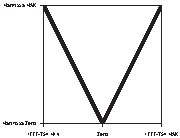
\includegraphics[page=1]{Number line.pdf}
\end{adjustbox}
\end{center}

\ppara{FIG. \ref{fig:ieee_number_line} illustrates the IEEE-754 sign-magnitude representation, highlighting the fundamental discontinuity that occurs at zero. The visualization shows how every numerical value has an opposite representation—positive and negative—that differ only by the sign bit, creating a mirrored duplicate of the entire number line. This includes cases like zero, which exists as both +0 and -0, despite representing the same mathematical value. This sign-magnitude approach creates a discontinuity at zero and introduces significant branching complexity in numerical operations, requiring separate code paths for different sign combinations and explicit testing of the sign bit for most arithmetic operations.}

\begin{lstlisting}[caption={Two's Complement Representation}, label={fig:spirix_number_line}]
\end{lstlisting}
\begin{center}
\begin{minipage}{0.48\textwidth}
  \centering
  \begin{adjustbox}{valign=t,width=\linewidth}
  \includegraphics[page=2]{Number line.pdf}
  \end{adjustbox}
\end{minipage}
\hfill
\begin{minipage}{0.48\textwidth}
  \centering
  \begin{adjustbox}{valign=t,width=\linewidth}
  \includegraphics[page=3]{Number line.pdf}
  \end{adjustbox}
\end{minipage}
\end{center}

\ppara{FIG. \ref{fig:spirix_number_line}A presents a linear view of the invention's continuous two's complement representation. Unlike IEEE-754, the invention achieves a completely continuous number space where values wrap around to maintain mathematical relationships across the entire range, eliminating the discontinuity at zero. This continuity enables operations to cross the zero boundary without any special handling or branching.}

\ppara{FIG. \ref{fig:spirix_number_line}B shows a vertically rotated perspective of the same representation, mapping values from fraction MAX/2+1 at the bottom to fraction MAX/2 at the top, with zero naturally landing in the middle. This visualization highlights how zero is now a contiguous value in the number line rather than as a special case.}

\subsection*{Core Configuration Definitions}

\ppara{The Scalar and Circle configurations form the core of the system. The following definitions outline their structure and representation:}

\begin{lstlisting}[style=rust, caption={Scalar Type Definition}, label={fig:scalar_structure}]
pub struct Scalar<F: Integer, E: Integer> {
	/// The normalized fraction component representing the significand.
	/// The fraction size determines the precision of the value.
	/// The N (prefix bit) pattern determines the number's state
	/// (normal, exploded, vanished, Zero or undefined/unimplemented).
	pub fraction: F,

	/// The exponent component determining the scale of the value/phase.
	/// The exponent size determines the range of the value/phase.
	/// When equal to AMBIGUOUS_EXPONENT, indicates an escaped phase
	/// (exploded, vanished, undefined/unimplemented or Zero).
	pub exponent: E,
}
\end{lstlisting}

\ppara{FIG. \ref{fig:scalar_structure} presents the implementation of the Scalar type, the invention's representation for real numbers. The structure shows the two primary components: a normalized two's complement fraction that determines precision, and an unbiased two's complement exponent that determines range. The type is parameterized to allow independent selection of fraction and exponent sizes according to application requirements.}

\begin{lstlisting}[style=rust, caption={Circle Type Definition}, label={fig:circle_structure}]
pub struct Circle<F: Integer, E: Integer> {
	/// The real phase representing the real part of the complex number.
	/// The normalization level of this component indicates current state
	/// (normal, exploded, vanished, undefined/unimplemented, Zero).
	pub real: F,

	/// The imaginary component representing the phase of i.
	/// The normalization level of this component indicates current state
	/// (normal, exploded, vanished, undefined/unimplemented, Zero).
	pub imaginary: F,

	/// The shared exponent component determining the scale of both phases.
	/// When equal to AMBIGUOUS_EXPONENT, indicates an escaped phase
	/// (exploded, vanished, undefined or Zero).
	pub exponent: E,
}
\end{lstlisting}

\ppara{FIG. \ref{fig:circle_structure} illustrates the Circle type definition for complex numbers. The structure contains real and imaginary fractions sharing a common exponent, enabling efficient complex arithmetic operations while maintaining mathematical consistency. Like the Scalar, Circle is parameterized to allow customization of precision and range.}

\begin{lstlisting}[style=rust, caption={Where fraction: F and exponent: E are any sized integer}, label={fig:integer}]
impl Integer for i8 {}
impl Integer for i16 {}
impl Integer for i32 {}
impl Integer for i64 {}
impl Integer for i128 {}
\end{lstlisting}

\ppara{FIG. \ref{fig:integer} demonstrates how the system abstracts over integer types. While the implementation shown uses all of Rust's native signed integer sizes (i8 thru i128) for illustration, the system can work with any arbitrary-sized integers for both fraction and exponent components. For example, custom integer sizes like <i12,i5> would be a perfectly valid implementation. This flexibility enables applications to precisely tune configurations based on their specific precision and range requirements.}

\begin{lstlisting}[caption={FE Type Configurations - Precision vs. Range}, label={fig:spirix_configurations}]
\end{lstlisting}
\begin{table}[ht]
\centering
\renewcommand{\arraystretch}{1.5}
\begin{tabular}{|c|c|c|c|c|c|}
\hline
\multirow{2}{*}{\textbf{Range}} & \multicolumn{5}{c|}{\textbf{Precision (Fraction Bits)}} \\
\cline{2-6}
 & \textbf{F3} & \textbf{F4} & \textbf{F5} & \textbf{F6} & \textbf{F7} \\
 & \small{2.2 digits} & \small{4.6 digits} & \small{9.4 digits} & \small{19 digits} & \small{38.3 digits} \\
\hline
\textbf{E3} & F3E3 & F4E3 & F5E3 & F6E3 & F7E3 \\
\small{$\approx 10^{\pm2.1}$} & \small{$\langle$i8, i8$\rangle$} & \small{$\langle$i16, i8$\rangle$} & \small{$\langle$i32, i8$\rangle$} & \small{$\langle$i64, i8$\rangle$} & \small{$\langle$i128, i8$\rangle$} \\
\hline
\textbf{E4} & F3E4 & F4E4 & F5E4 & F6E4 & F7E4 \\
\small{$\approx 10^{\pm4.5}$} & \small{$\langle$i8, i16$\rangle$} & \small{$\langle$i16, i16$\rangle$} & \small{$\langle$i32, i16$\rangle$} & \small{$\langle$i64, i16$\rangle$} & \small{$\langle$i128, i16$\rangle$} \\
\hline
\textbf{E5} & F3E5 & F4E5 & F5E5 & F6E5 & F7E5 \\
\small{$\approx 10^{\pm9.3}$} & \small{$\langle$i8, i32$\rangle$} & \small{$\langle$i16, i32$\rangle$} & \small{$\langle$i32, i32$\rangle$} & \small{$\langle$i64, i32$\rangle$} & \small{$\langle$i128, i32$\rangle$} \\
\hline
\textbf{E6} & F3E6 & F4E6 & F5E6 & F6E6 & F7E6 \\
\small{$\approx 10^{\pm18.9}$} & \small{$\langle$i8, i64$\rangle$} & \small{$\langle$i16, i64$\rangle$} & \small{$\langle$i32, i64$\rangle$} & \small{$\langle$i64, i64$\rangle$} & \small{$\langle$i128, i64$\rangle$} \\
\hline
\textbf{E7} & F3E7 & F4E7 & F5E7 & F6E7 & F7E7 \\
\small{$\approx 10^{\pm38.2}$} & \small{$\langle$i8, i128$\rangle$} & \small{$\langle$i16, i128$\rangle$} & \small{$\langle$i32, i128$\rangle$} & \small{$\langle$i64, i128$\rangle$} & \small{$\langle$i128, i128$\rangle$} \\
\hline
\end{tabular}
\end{table}

\ppara{FIG. \ref{fig:spirix_configurations} presents the matrix of valid FE type combinations, showing how precision (columns) and range (rows) can be independently configured. The table provides approximate decimal digit precision and magnitude range for each configuration.}

\ppara{Scalar values are calculated as:}
\ppara{$value = fraction \times 2^{exponent}$}

\ppara{Circle values have real and imaginary phases sharing a common exponent:}
\ppara{$value = (real + imaginary \times i) \times 2^{exponent}$}

\subsection*{Normalization Levels and Bit Patterns}

\begin{lstlisting}[caption={Normalization Levels and Bit Patterns}, label={fig:normalization_levels}]
\end{lstlisting}
\begin{figure}[ht]
\centering
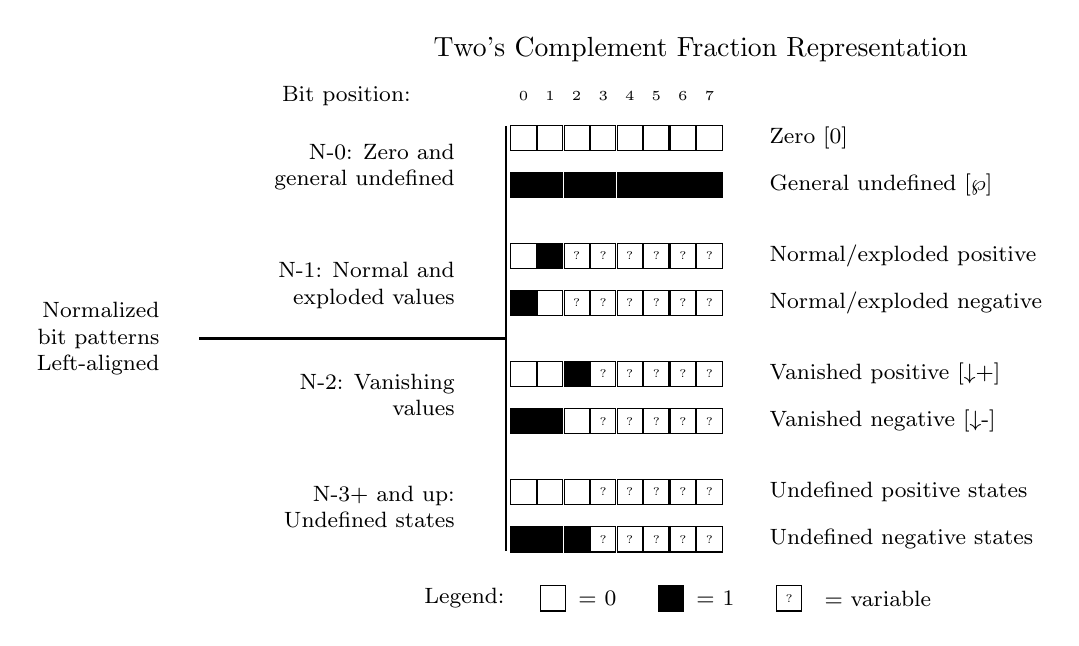
\begin{tikzpicture}[
    scale=0.75,
    every node/.style={font=\footnotesize},
    bit/.style={minimum width=0.4cm, minimum height=0.4cm, draw, anchor=center},
    highlight/.style={fill=black, text=white},
    empty/.style={fill=white},
    ]
    
    % Title
    \node at (4, 9.5) {\normalsize Two's Complement Fraction Representation};
    
    % Bit position markers
    \node[align=right] at (-2, 8.7) {Bit position:};
    \foreach \i in {0,...,7} {
        \node at (\i*0.45+1, 8.7) {\tiny \i};
    }
    
    % N-0: Zero and general undefined
    \node[align=right, anchor=east] at (0, 7.5) {N-0: Zero and\\general undefined};
    
    % Zero pattern
    \foreach \i in {0,...,7} {
        \node[bit, empty, scale=0.8] at (\i*0.45+1, 8) {};
    }
    \node[align=left, anchor=west] at (5, 8) {Zero [0]};
    
    % Undefined pattern
    \foreach \i in {0,...,7} {
        \node[bit, highlight, scale=0.8] at (\i*0.45+1, 7.2) {};
    }
    \node[align=left, anchor=west] at (5, 7.2) {General undefined [$\wp$]};
    
    % N-1: Normal and exploded values
    \node[align=right, anchor=east] at (0, 5.5) {N-1: Normal and\\exploded values};
    
    % Positive normal/exploded pattern
    \node[bit, empty, scale=0.8] at (1, 6) {};
    \node[bit, highlight, scale=0.8] at (1.45, 6) {};
    \foreach \i in {2,...,7} {
        \node[bit, scale=0.8] at (\i*0.45+1, 6) {\tiny?};
    }
    \node[align=left, anchor=west] at (5, 6) {Normal/exploded positive};
    
    % Negative normal/exploded pattern
    \node[bit, highlight, scale=0.8] at (1, 5.2) {};
    \node[bit, empty, scale=0.8] at (1.45, 5.2) {};
    \foreach \i in {2,...,7} {
        \node[bit, scale=0.8] at (\i*0.45+1, 5.2) {\tiny?};
    }
    \node[align=left, anchor=west] at (5, 5.2) {Normal/exploded negative};
    
    % N-2: Vanishing values
    \node[align=right, anchor=east] at (0, 3.65) {N-2: Vanishing\\values};
    
    % Positive vanished pattern
    \node[bit, empty, scale=0.8] at (1, 4) {};
    \node[bit, empty, scale=0.8] at (1.45, 4) {};
    \node[bit, highlight, scale=0.8] at (1.9, 4) {};
    \foreach \i in {3,...,7} {
        \node[bit, scale=0.8] at (\i*0.45+1, 4) {\tiny?};
    }
    \node[align=left, anchor=west] at (5, 4) {Vanished positive [$\downarrow$+]};
    
    % Negative vanished pattern
    \node[bit, highlight, scale=0.8] at (1, 3.2) {};
    \node[bit, highlight, scale=0.8] at (1.45, 3.2) {};
    \node[bit, empty, scale=0.8] at (1.9, 3.2) {};
    \foreach \i in {3,...,7} {
        \node[bit, scale=0.8] at (\i*0.45+1, 3.2) {\tiny?};
    }
    \node[align=left, anchor=west] at (5, 3.2) {Vanished negative [$\downarrow$-]};
    
    % N-3+: Specific undefined states
    \node[align=right, anchor=east] at (0, 1.75) {N-3+ and up:\\Undefined states};
    
    % Positive undefined patterns
    \node[bit, empty, scale=0.8] at (1, 2) {};
    \node[bit, empty, scale=0.8] at (1.45, 2) {};
    \node[bit, empty, scale=0.8] at (1.9, 2) {};
    \foreach \i in {3,...,7} {
        \node[bit, scale=0.8] at (\i*0.45+1, 2) {\tiny?};
    }
    \node[align=left, anchor=west] at (5, 2) {Undefined positive states};
    
    % Negative undefined patterns
    \node[bit, highlight, scale=0.8] at (1, 1.2) {};
    \node[bit, highlight, scale=0.8] at (1.45, 1.2) {};
    \node[bit, highlight, scale=0.8] at (1.9, 1.2) {};
    \foreach \i in {3,...,7} {
        \node[bit, scale=0.8] at (\i*0.45+1, 1.2) {\tiny?};
    }
    \node[align=left, anchor=west] at (5, 1.2) {Undefined negative states};
    
    \draw [thick] (0.7,8.2) -- (0.7,1);
    \draw [thick] (0.7,4.6) -- (-4.5,4.6);
    \node [align=right, anchor=east] at (-5, 4.6) {Normalized\\bit patterns\\Left-aligned};
    
    % Legend
    \node at (0, 0.2) {Legend:};
    \node[bit, empty, scale=0.8] at (1.5, 0.2) {};
    \node at (2.25, 0.2) {= 0};
    \node[bit, highlight, scale=0.8] at (3.5, 0.2) {};
    \node at (4.25, 0.2) {= 1};
    \node[bit, scale=0.8] at (5.5, 0.2) {\tiny?};
    \node at (7, 0.2) {= variable};
    
\end{tikzpicture}
\end{figure}

\ppara{FIG. \ref{fig:normalization_levels} visualizes the invention's left-aligned normalization scheme, showing how specific bit patterns in the most significant positions encode different numeric states. The illustration demonstrates how normal values, exploded values, vanished values, and various undefined states are represented thru distinct bit patterns, where $\blacksquare$ represents binary 1s, $\square$ represents binary 0s, and {\tiny?} represents variable bits holding numeric data. This approach enables exponent-only single check state detection without extensive branching, unlike IEEE-754 which requires explicit checking of exponent values and various fraction and sign bit combinations. The normalization scheme supports any number of N-levels from N-0 up to the fraction bit size, allowing for future extension of states and capabilities as needed. This extensibility ensures that the system can evolve to handle new mathematical implementations or domain-specific undefined states while maintaining backward compatibility with existing implementations.}

\subsection*{Undefined States}

\ppara{One of the key innovations in the invention is the preservation of error information thru dedicated undefined patterns in the upper bits. Unlike IEEE-754's single NaN value, the system uses specific bit patterns to track the cause of undefined operations:}

\begin{lstlisting}[style=rust, caption={Excerpt of Undefined State Definitions}, label={fig:undefined}]
// L3 Basic operators
/// ¡$\square\square\square\blacksquare\blacksquare\blacksquare\blacksquare\blacksquare$¡
pub const EXPLODED_PLUS_EXPLODED: Undefined = Undefined {
	prefix: 0b00011111u8 as i8,
	symbol: "¡$\wp$¡ ¡$\uparrow$¡+¡$\uparrow$¡",
	description: "Exploded value addition with exploded value",
};
/// ¡$\blacksquare\blacksquare\blacksquare\square\square\square\square\square$¡
pub const EXPLODED_MINUS_EXPLODED: Undefined = Undefined {
	prefix: 0b11100000u8 as i8,
	symbol: "¡$\wp$¡ ¡$\uparrow$¡-¡$\uparrow$¡",
	description: "Exploded value subtraction with exploded value",
};
/// ¡$\square\square\square\blacksquare\blacksquare\blacksquare\blacksquare\square$¡
pub const VANISHED_PLUS_VANISHED: Undefined = Undefined {
	prefix: 0b00011110u8 as i8,
	symbol: "¡$\wp$¡ ¡$\downarrow$¡+¡$\downarrow$¡",
	description: "Vanished value addition with vanished value",
};
/// ¡$\blacksquare\blacksquare\blacksquare\square\square\square\square\blacksquare$¡
pub const VANISHED_MINUS_VANISHED: Undefined = Undefined {
	prefix: 0b11100001u8 as i8,
	symbol: "¡$\wp$¡ ¡$\downarrow$¡-¡$\downarrow$¡",
	description: "Vanished value subtraction with vanished value",
};
// L4 Powers and roots
/// ¡$\square\square\square\square\blacksquare\blacksquare\blacksquare\blacksquare$¡
pub const EXPLODED_POWER: Undefined = Undefined {
	prefix: 0b00001111u8 as i8,
	symbol: "¡$\wp$¡ ¡$\uparrow$¡^",
	description: "Exploded value raised to power",
};
/// ¡$\blacksquare\blacksquare\blacksquare\blacksquare\square\square\square\square$¡
pub const VANISHED_POWER: Undefined = Undefined {
	prefix: 0b11110000u8 as i8,
	symbol: "¡$\wp$¡ ¡$\downarrow$¡^",
	description: "Vanished value raised to power",
};
/// ¡$\square\square\square\square\blacksquare\blacksquare\blacksquare\square$¡
pub const POWER_EXPLODED: Undefined = Undefined {
	prefix: 0b00001110u8 as i8,
	symbol: "¡$\wp$¡ ^¡$\uparrow$¡",
	description: "Value raised to exploded power",
};

// L5 Logarithms
/// ¡$\square\square\square\square\square\blacksquare\blacksquare\blacksquare$¡
pub const EXPLODED_LOG: Undefined = Undefined {
	prefix: 0b00000111u8 as i8,
	symbol: "¡$\wp$¡ ¡$\uparrow$¡@",
	description: "Logarithm of exploded value",
};
/// ¡$\blacksquare\blacksquare\blacksquare\blacksquare\blacksquare\square\square\square$¡
pub const VANISHED_LOG: Undefined = Undefined {
	prefix: 0b11111000u8 as i8,
	symbol: "¡$\wp$¡ ¡$\downarrow$¡@",
	description: "Logarithm of vanished value",
};
/// ¡$\square\square\square\square\square\blacksquare\blacksquare\square$¡
pub const LOG_EXPLODED: Undefined = Undefined {
	prefix: 0b00000110u8 as i8,
	symbol: "¡$\wp$¡ @¡$\uparrow$¡",
	description: "Logarithm with exploded base",
};

// L6 Sine/Cosine
/// ¡$\square\square\square\square\square\square\blacksquare\blacksquare$¡
pub const SINE: Undefined = Undefined {
	prefix: 0b00000011u8 as i8,
	symbol: "¡$\wp$¡ s",
	description: "Sine of value with imprecise period position",
};
/// ¡$\blacksquare\blacksquare\blacksquare\blacksquare\blacksquare\blacksquare\square\square$¡
pub const COSINE: Undefined = Undefined {
	prefix: 0b11111100u8 as i8,
	symbol: "¡$\wp$¡ c",
	description: "Cosine of value with imprecise period position",
};

// L7 Tangent and extensions
/// ¡$\square\square\square\square\square\square\square\blacksquare$¡
pub const TANGENT: Undefined = Undefined {
	prefix: 0b00000001u8 as i8,
	symbol: "¡$\wp$¡ t",
	description: "Tangent of value with imprecise period position",
};
\end{lstlisting}

\ppara{FIG. \ref{fig:undefined} illustrates the invention's hierarchy of undefined states. Unlike IEEE-754's single NaN representation, the system employs specific bit patterns to encode the precise cause of undefined operations. The figure shows how each undefined state is defined with a unique prefix, a symbol (like "℘ $\uparrow$+$\uparrow$"), and a descriptive name. The system preserves the first cause of undefined operations during propagation, for example when computing "0$\^{}$0 + 0/0 = ℘0$\^{}$0" maintains the initial undefined cause (Zero raised to Zero power) thruout subsequent operations. By assigning different undefined operations with unique states, the invention enables precise error tracking, allowing users to trace numerical issues to their origin rather than encountering a generic "Not a Number" error.}

\subsection*{Subtractive and Multiplicative Consistency Without Denormals}

\ppara{A significant innovation in the invention is how it maintains mathematical consistency and subtractive equality properties without requiring denormal numbers. In IEEE-754, denormal numbers were introduced to address a specific edge case: maintaining the mathematical property that x = y if and only if x - y = 0. Without denormals, IEEE-754 encounters situations where two distinct representable numbers subtract to produce zero because their difference would be too small to represent as a normalized number and truncated to zero, potentially causing unexpected behavior in algorithms that rely on this mathematical property.}

\ppara{The invention's two's complement representation with the "vanished" state solves this problem using a different mechanism. When a value becomes too small for normal representation, it transitions to a vanished state that preserves its sign information. Unlike IEEE-754 denormals, which represent specific tiny values with reduced precision, the invention's vanished values represent a categorical state of "too small to represent normally." This approach maintains the critical property that equal values always have a zero difference, while eliminating the implementation complexity and performance penalties associated with denormal handling.}

\ppara{Consider two values a and b that are very close but not identical. Their difference a - b will either be a normal value (if the difference is representable) or a vanished value (if the difference is too small for normal representation). In either case, the difference will be non-zero, preserving the property that a = b if and only if a - b = 0. Significantly, this holds true without requiring the extensive special case handling that denormals introduce.}

\ppara{The invention also improves mathematical consistency in multiplicative and reciprocal operations at extremes of representable ranges. Unlike IEEE-754, which allows products of non-zero values to become zero when they underflow, the invention guarantees that the product of any two non-zero values always produces a non-zero result, preserving fundamental mathematical principles. Similarly, reciprocal operations maintain mathematical coherence: 1/0 produces an infinite result with a specific bit pattern, while 1/vanished produces an exploded result with the appropriate sign, ensuring that information about magnitude limits is preserved thruout calculations.}

\subsection*{IEEE-754 Numerical Operations}

\ppara{In IEEE-754, floating-point operations follow a complicated sequence of steps with numerous special case handling requirements. The sign-magnitude representation necessitates explicit sign bit testing for virtually all operations. For basic arithmetic functions like addition and subtraction, the processor must first examine sign bits to determine whether to perform addition or subtraction of magnitudes, followed by potential sign adjustment of the result. This sign-dependent processing path creates a fundamental bifurcation in the execution flow.}

\ppara{Multiplication and division operations in IEEE-754 similarly require sign bit extraction and separate processing. The sign of the result is determined by XORing the sign bits of operands, while magnitude calculations proceed independently. Special values like NaN, infinities, zeros (both positive and negative), and subnormal numbers each trigger distinct processing paths with their own rules and exceptions.}

\ppara{Transcendental functions in IEEE-754 contain extensive special case handling for boundary values. Functions like logarithm, sine, and tangent must implement separate processing for inputs near zero, extremely large values, negative numbers, and special values. Each of these cases introduces additional branching, often requiring multiple comparison operations and conditional jumps that impact instruction pipeline efficiency and predictability. This branching complexity becomes particularly problematic in SIMD (Single Instruction Multiple Data) processing environments, where divergent execution paths across data lanes can significantly degrade performance.}
\newpage
\begin{lstlisting}[caption={IEEE-754 Subtraction Flowchart}, label={fig:ieee_subtract_flowchart}]
\end{lstlisting}
\begin{figure}[htbp]
  \centering
  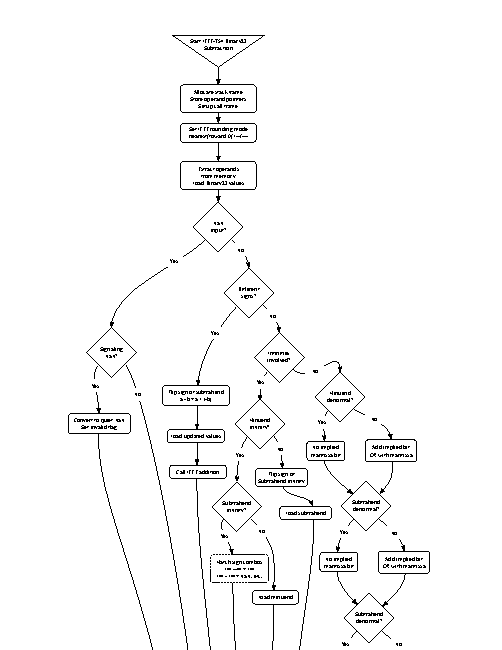
\includepdf[pages=1, scale=0.85]{IEEE subtract flowchart.pdf}
\end{figure}
\newpage
\begin{figure}[htbp]
  \centering
  \includepdf[pages=2, scale=0.85]{IEEE subtract flowchart.pdf}
\end{figure}
\newpage
\begin{figure}[htbp]
  \centering
  \includepdf[pages=3, scale=0.85]{IEEE subtract flowchart.pdf}
\end{figure}
\newpage

\ppara{FIG. \ref{fig:ieee_subtract_flowchart} details the elaborate control flow required for IEEE-754 subtraction operations. The flowchart reveals numerous branching paths needed to handle different sign combinations, exponent comparisons, and special value cases, illustrating the implementation complexity that results from IEEE-754's disjoint representation of signs and fractions.}

\begin{lstlisting}[style=rust, caption={Annotated Binary32 Normal Case Subtraction Instruction Trace}, label={fig:ieee_subtract}]
; Main Subtraction Fuction Entry Point
[001]sub rsp, 0x58                 ; Allocate 88 bytes on the stack
[002]mov qword ptr [rsp 0x8], rdi  ; Store first parameter (pointer to first value)
[003]mov al, dl                    ; Move the 3rd parameter (lower byte) to al
[004]mov dword ptr [rsp 0x18], esi ; Store second parameter (second value)
[005]mov ecx, dword ptr [rsp 0x18] ; Load second Binary32 value into ecx
[006]mov dword ptr [rsp 0x14], ecx ; Store second Binary32 value at rsp+20
[007]mov byte ptr [rsp 0x1f], al   ; Store lower byte of 3rd parameter at rsp+31
[008]mov qword ptr [rsp 0x30], rdi ; Move first parameter
[009]lea rax, ptr [rip 0x3d6e9]    ; Load effective address
[010]lea rdi, ptr [rsp 0x1f]       ; Load address of next function into rdi
[011]call rax                      ; Call function at address in rax

; Set Rounding Mode
[012]push rax                 ; Save rax register
[013]mov qword ptr [rsp], rdi ; Store rdi at top of stack
[014]call 0x558bdf671e20      ; Call function to set rounding mode

; Convert Rounding Mode to Float Format
[015]mov qword ptr [rsp-0x8], rdi      ; Store rdi at rsp-8
[016]movzx eax, byte ptr [rdi]         ; Zero-extend byte at [rdi] into eax
[017]mov qword ptr [rsp-0x18], rax     ; Store extended value at rsp-24
[018]mov rax, qword ptr [rsp-0x18]     ; Load value from rsp-24 into rax
[019]lea rcx, ptr [rip 0x452af]        ; Load effective address (jump table?)
[020]movsxd rax, dword ptr [rcx rax*4] ; Load and sign-extend value from jump table
[021]add rax, rcx                      ; Add base address to jump offset
[022]jmp rax                           ; Jump to the calculated address
[023]mov byte ptr [rsp-0x9], 0x0       ; Set byte at rsp-9 to 0
[024]jmp 0x558bdf671e65                ; Jump to function epilogue
[025]mov al, byte ptr [rsp-0x9]        ; Load byte from rsp-9 into al
[026]ret                               ; Return from function

; Set Rounding Mode
[027]movzx edi, al                ; Zero-extend al into edi
[028]call qword ptr [rip 0x5bf45] ; Call function pointer at rip+0x5bf45

; Rounding Mode Helper
[029]push rbp                     ; Save base pointer
[030]mov rbp, rsp                 ; Set new base pointer
[031]push rbx                     ; Save rbx register
[032]sub rsp, 0x8                 ; Allocate 8 bytes on stack
[033]mov ebx, edi                 ; Store first parameter in ebx
[034]mov rax, qword ptr fs:[0x0]  ; Load value from fs segment
[035]lea rax, ptr [rax-0x4f]      ; Calculate address at fs:0 - 79
[036]mov byte ptr [rax], bl       ; Store lowest byte of ebx at calculated address
[037]mov rbx, qword ptr [rbp-0x8] ; Restore rbx
[038]leave                        ; Restore stack and base pointer
[039]ret                          ; Return from function

; Set Rounding Mode (continued)
[040]pop rax ; Restore rax
[041]ret     ; Return from function

; Main Subtraction Function (continued)
[042]jmp 0x558bdf63473a            ; Jump to next part of subtraction function
[043]mov rax, qword ptr [rsp 0x8]  ; Load pointer to first Binary32 from rsp+8
[044]mov eax, dword ptr [rax]      ; Load value of first Binary32 into eax
[045]mov dword ptr [rsp 0x28], eax ; Store first Binary32 at rsp+40
[046]lea rdi, ptr [rsp 0x14]       ; Load address of second value into rdi
[047]call 0x558bdf6346e0           ; Call function to borrow memory value

; Borrow Memory Value
[048]mov rax, rdi                 ; Copy input parameter to rax
[049]mov qword ptr [rsp-0x8], rax ; Store rax at rsp-8
[050]ret                          ; Return from function

; Main Subtraction Function (continued)
[051]mov qword ptr [rsp], rax      ; Store return value at top of stack
[052]jmp 0x558bdf634755            ; Jump to next part of subtraction
[053]mov rax, qword ptr [rsp]      ; Load pointer from stack into rax
[054]mov eax, dword ptr [rax]      ; Load value at pointer into eax
[055]mov dword ptr [rsp 0x2c], eax ; Store second Binary32 at rsp+44
[056]mov eax, dword ptr [rsp 0x28] ; Load first Binary32 into eax
[057]mov dword ptr [rsp 0x4c], eax ; Store first Binary32 at rsp+76
[058]mov edi, dword ptr [rsp 0x4c] ; Load first value into edi
[059]mov eax, dword ptr [rsp 0x2c] ; Load second Binary32 into eax
[060]mov dword ptr [rsp 0x50], eax ; Store second Binary32 at rsp+80
[061]mov esi, dword ptr [rsp 0x50] ; Load second value into esi
[062]call qword ptr [rip 0x9906b]  ; Call function for low-level

; Low-level Float Subtraction
[063]push rbp            ; Save base pointer
[064]mov rbp, rsp        ; Set new base pointer
[065]mov eax, edi        ; Copy first Binary32 to eax
[066]mov edx, esi        ; Copy second Binary32 to edx
[067]xor esi, edi        ; XOR the two Binary32 values
[068]js 0x558bdf671e83   ; Jump if sign bit is set (opposing signs)
[069]mov rsi, rdx        ; Copy second Binary32 to rsi
[070]mov rdi, rax        ; Copy first Binary32 to rdi
[071]call 0x558bdf6721a9 ; Call function to add float magnitudes

; Add Float Magnitudes
[072]push rbp            ; Save base pointer
[073]mov rbp, rsp        ; Set new base pointer
[074]mov rcx, rdi        ; Copy first Binary32 to rcx
[075]shr rcx, 0x17       ; Shift right by 23 bits (extract exponent)
[076]movzx ecx, cl       ; Zero-extend lowest byte to get 8-bit exponent
[077]mov r9, rcx         ; Copy exponent to r9
[078]mov r10, rdi        ; Copy first Binary32 to r10
[079]and r10d, 0x7fffff  ; Mask to get mantissa (23 bits)
[080]mov rax, rsi        ; Copy second Binary32 to rax
[081]shr rax, 0x17       ; Shift right by 23 bits (extract exponent)
[082]movzx eax, al       ; Zero-extend lowest byte to get 8-bit exponent
[083]mov rdx, rsi        ; Copy second Binary32 to rdx
[084]and edx, 0x7fffff   ; Mask to get mantissa (23 bits)
[085]mov r11, rcx        ; Copy first exponent to r11
[086]sub r11, rax        ; Subtract exponents (for comparing magnitude)
[087]jnz 0x558bdf67224f  ; Jump if exponents are different
[088]mov r8d, edi        ; Copy first Binary32 to r8d
[089]shr r8d, 0x1f       ; Shift right by 31 bits (extract sign bit)
[090]shl r10, 0x6        ; Shift first mantissa left by 6 bits (normalize)
[091]shl rdx, 0x6        ; Shift second mantissa left by 6 bits (normalize)
[092]test r11, r11       ; Test if exponent difference is Zero
[093]js 0x558bdf6722c4   ; Jump if exponent difference is negative
[094]cmp rax, 0xff       ; Check for NaN/Infinity
[095]jz 0x558bdf67230b   ; Jump if second number is NaN or Infinity
[096]test rcx, rcx       ; Test if first exponent is Zero
[097]mov esi, 0x20000000 ; Set esi to 0x20000000 (implied 1 for normal numbers)
[098]cmovz rsi, r10      ; True for normals, false for subnormal
[099]mov rdi, rax        ; Copy second exponent to rdi
[100]sub rdi, rcx        ; Calculate exponent difference
[101]add rsi, r10        ; Add implied 1 to first mantissa
[102]cmp rdi, 0x1e       ; Compare exponent difference with 30
[103]jnbe 0x558bdf672327 ; Jump if difference is not within range
[104]mov ecx, edi        ; Copy exponent difference to ecx
[105]neg ecx             ; Negate exponent difference
[106]mov r9d, esi        ; Copy first mantissa with implied 1 to r9d
[107]shl r9d, cl         ; Shift left by exponent difference
[108]test r9d, r9d       ; Test if shifted value is Zero
[109]setnz r10b          ; Set r10b to 1 if not Zero, 0 if Zero
[110]movzx r10d, r10b    ; Zero-extend r10b to r10d
[111]mov ecx, edi        ; Copy exponent difference to ecx
[112]shr esi, cl         ; Shift first mantissa right by exponent difference
[113]or r10d, esi        ; Combine shifted bits with sticky bit
[114]mov r10d, r10d      ; Clear upper 32 bits of r10
[115]mov r9, rax         ; Copy second exponent to r9
[116]jmp 0x558bdf6722a3  ; Jump to next part of float addition
[117]lea rdx, ptr [r10 rdx*1 0x20000000] ; Calculate sum of mantissas
[118]cmp rdx, 0x3fffffff ; Check if result needs normalization
[119]jnbe 0x558bdf67220e ; Jump if normalization needed
[120]movzx edi, r8b      ; Zero-extend sign bit to edi
[121]mov rsi, r9         ; Copy exponent to rsi
[122]call 0x558bdf671f65 ; Call function to round and pack to Binary32 format

; Round and Pack to Binary32 Format
[123]push rbp                      ; Save base pointer
[124]mov rbp, rsp                  ; Set new base pointer
[125]push r15                      ; Save r15 register
[126]push r14                      ; Save r14 register
[127]push r13                      ; Save r13 register
[128]push r12                      ; Save r12 register
[129]push rbx                      ; Save rbx register
[130]sub rsp, 0x18                 ; Allocate 24 bytes on stack
[131]mov r15d, edi                 ; Store sign bit in r15d
[132]mov dword ptr [rbp-0x34], edi ; Store sign bit at rbp-52
[133]mov rbx, rsi                  ; Store exponent in rbx
[134]mov r13, rdx                  ; Store mantissa in r13
[135]mov rax, qword ptr fs:[0x0]   ; Load value from fs segment
[136]lea rax, ptr [rax-0x4f]       ; Calculate address at fs:0 - 79
[137]movzx r14d, byte ptr [rax]    ; Load rounding mode into r14d
[138]test r14b, r14b               ; Test if rounding mode is 0 (to nearest)
[139]setz byte ptr [rbp-0x40]      ; Set flag at rbp-64 if rounding mode is 0
[140]mov r12d, 0x40                ; Set r12d to 64 (used for rounding)
[141]test r14b, 0xfb               ; Test rounding mode against 0xfb
[142]jz 0x558bdf671fc9             ; Jump if specific rounding mode
[143]mov r15d, r13d                ; Copy mantissa to r15d
[144]and r15d, 0x7f                ; Mask with 0x7f (7 least significant bits)
[145]mov dword ptr [rbp-0x38], ebx ; Store exponent at rbp-56
[146]cmp ebx, 0xfc                 ; Compare exponent with 0xfc
[147]jbe 0x558bdf672000            ; Jump if exponent <= 0xfc
[148]movzx r12d, r12b              ; Zero-extend r12b to r12d
[149]add r12, r13                  ; Add mantissa to r12
[150]shr r12, 0x7                  ; Shift right by 7 bits (rounding)
[151]test r15b, r15b               ; Test if lower 7 bits are Zero
[152]jnz 0x558bdf6720ec            ; Jump if lower 7 bits are not Zero
[153]mov rax, qword ptr fs:[0x0]   ; Load value from fs segment
[154]lea rax, ptr [rax-0x50]       ; Calculate address at fs:0 - 80
[155]or byte ptr [rax], 0x1        ; Set inexact flag
[156]cmp r14b, 0x6                 ; Compare rounding mode with 6
[157]jnz 0x558bdf672014            ; Jump if rounding mode is not 6
[158]cmp r15b, 0x40                ; Compare lower 7 bits with 0x40
[159]setz al                       ; Set al to 1 if equal, 0 if not
[160]movzx eax, al                 ; Zero-extend al to eax
[161]and rax, qword ptr [rbp-0x40] ; AND with rounding flag
[162]not rax                       ; Complement result
[163]and r12, rax                  ; Mask r12 with result
[164]mov eax, 0x0                  ; Set eax to 0
[165]cmovz rbx, rax                ; If Zero, set exponent to 0
[166]mov eax, dword ptr [rbp-0x34] ; Load sign bit into eax
[167]shl eax, 0x1f                 ; Shift sign bit to position 31
[168]shl ebx, 0x17                 ; Shift exponent to position 23-30
[169]add eax, ebx                  ; Combine sign and exponent
[170]mov eax, eax                  ; Clear upper 32 bits
[171]add rax, r12                  ; Add mantissa to result
[172]add rsp, 0x18                 ; Deallocate stack space
[173]pop rbx                       ; Restore rbx
[174]pop r12                       ; Restore r12
[175]pop r13                       ; Restore r13
[176]pop r14                       ; Restore r14
[177]pop r15                       ; Restore r15
[178]pop rbp                       ; Restore base pointer
[179]ret                           ; Return from function

; Add Float Magnitudes (epilogue)
[180]pop rbp ; Restore base pointer
[181]ret     ; Return from function

; Low-level Float Subtraction (epilogue)
[182]jmp 0x558bdf671e81 ; Jump to another part of function
[183]pop rbp            ; Restore base pointer
[184]ret                ; Return from function

; Main Subtraction Function (epilogue)
[185]mov dword ptr [rsp 0x54], eax ; Store result at rsp+84
[186]mov eax, dword ptr [rsp 0x54] ; Load result back into eax
[187]mov dword ptr [rsp 0x24], eax ; Store result at rsp+36
[188]mov eax, dword ptr [rsp 0x24] ; Load result back into eax
[189]mov dword ptr [rsp 0x20], eax ; Store result at rsp+32
[190]mov eax, dword ptr [rsp 0x20] ; Load result back into eax
[191]add rsp, 0x58                 ; Deallocate 88 bytes from stack
[192]ret                           ; Return from function

\end{lstlisting}

\ppara{The IEEE-754 subtraction implementation shown above requires approximately 192 machine instructions with complex branching logic for even simple cases. This trace includes 7 function calls, 6 unconditional jumps, 10 conditional branches, and 7 returns across multiple abstraction layers. Each branch introduces potential pipeline stalls and prediction failures in modern processors, particularly impacting SIMD performance where lane divergence can severely degrade thruput. The extensive special-case handling required by IEEE-754's separate sign bit and fragmented representation creates this branching complexity, resulting in less predictable execution paths and increased computational overhead compared to the invention's approach.}

\subsection*{The Invention's Numerical Operations}

\ppara{In contrast to IEEE-754, the invention's implementation maintains a streamlined approach with only two main execution paths: one for normal values and one for ambiguous cases. This simplification eliminates the need for sign-specific logic and special case explosion, resulting in more predictable execution paths and improved performance, especially in SIMD environments.}
\newpage
\begin{lstlisting}[caption={Scalar Subtraction Flowchart}, label={fig:scalar_subtract_flowchart}]
\end{lstlisting}
\begin{figure}[htbp]
  \centering
  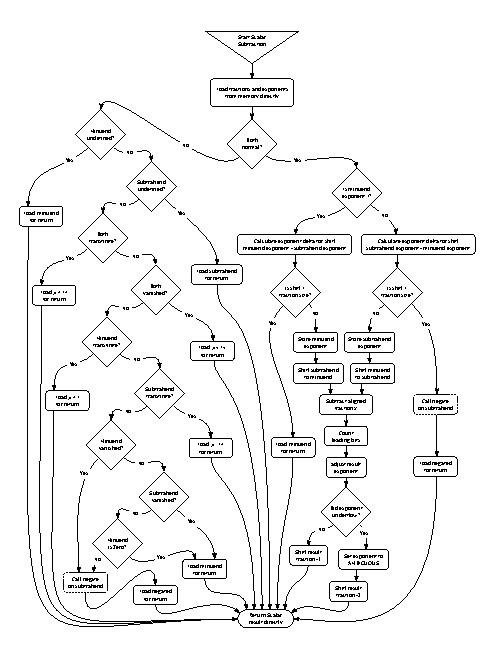
\includepdf[pages=1, scale=0.85]{Scalar subtract flowchart.pdf}
\end{figure}
\newpage

\ppara{FIG. \ref{fig:scalar_subtract_flowchart} illustrates the control flow of the invention's scalar subtraction. The diagram shows just two primary paths: one for normal values and one for ambiguous cases, with no jumps in the main path. This simpler structure directly results from the invention's continuous two's complement representation, which eliminates the need for dedicated sign handling and independent magnitudes.}

\begin{lstlisting}[style=rust, caption={Assembly Implementation of Scalar Subtraction}, label={fig:scalar_subtract}]
; ScalarF5E4-ScalarF5E4 handwritten by Nick Spiker fractaldecoder@proton.me
; Performs normal subtraction with 32-bit fractions and 16-bit exponents
; Input: Result pointer in rdi, Minuend in rsi, Subtrahend in rdx

; Register allocation:
; rax - a.fraction/result fraction (64-bit extended)
; rbx - b.fraction (64-bit extended)
; ecx - exponent difference/normalization shift
; r8d - a.exponent/result exponent
; r9d - b.exponent
; edx - leading bits counter

; Load values with sign extension
[01]movsx rax, dword ptr [rsi]  ; Load a.fraction
[02]movsx rbx, dword ptr [rdx]  ; Load b.fraction
[03]movsx r8d, word ptr [rsi+4] ; Load a.exponent
[04]movsx r9d, word ptr [rdx+4] ; Load b.exponent

; Check for ambiguous exponents
[05]cmp r8d, 0x8000      ; Compare with AMBIGUOUS_EXPONENT
[06]je ambiguous_handler ; Jump if a is ambiguous
[07]cmp r9d, 0x8000      ; Compare with AMBIGUOUS_EXPONENT
[08]je ambiguous_handler ; Jump if b is ambiguous

; Calculate exponent difference
[09]mov ecx, r8d ; Use ecx to store exponent diff
[10]sub ecx, r9d ; ecx = a.exp - b.exp
[11]js b_larger  ; Jump if b's exponent is larger

; Minuend has larger exponent
[12]cmp ecx, 32  ; Shift amount >= 32 bits?
[13]jge return ; If yes, b's contribution is negligible

; Perform shift and subtraction
[14]shl rax, cl       ; Align a to b
[15]sub rax, rbx      ; (a << diff) - b
[16]test rax, rax     ; Check if result is zero
[17]jz set_ambiguous  ; If zero, set exponent to AMBIGUOUS
[18]lea r8d, [r9d+32] ; Intermediary exponent=b.exp+offset

normalize:
[19]lzcnt edx, eax       ; Count leading zeros
[20]not rax              ; Invert for leading ones count
[21]lzcnt ecx, eax       ; Count leading ones (as zeros in inverted)
[22]not rax              ; Restore original value
[23]cmp edx, ecx         ; Compare leading zeros with leading ones
[24]cmovl edx, ecx       ; Take max (Leading Same Bits)
[25]dec edx              ; Offset for N-1 normalization
[26]shl rax, edx         ; Normalize to N-1 high bits
[27]shr rax, 32          ; Re-align to single-wide
[28]sub r8d, edx         ; Adjust result exponent by shift amount
[29]cmp r8d, 0x8001      ; Check result for underflow
[30]jl underflow_handler ; Jump if underflow detected

return:
[31]mov dword ptr [rdi], eax  ; Store result fraction
[32]mov word ptr [rdi+4], r8w ; Store result exponent
[33]ret

underflow_handler:
[34]shr rax, 1 ; Shift fraction to N-2 normalization

set_ambiguous:
[35]mov r8d, 0x8000 ; Set exponent to AMBIGUOUS_EXPONENT
[36]jmp return

b_larger:
[37]neg ecx         ; Convert negative diff to positive
[39]jge b_dominates ; If yes, a's contribution is negligible

; Perform shift and subtraction with b larger
[40]shl rbx, cl      ; Align b to a
[41]sub rax, rbx     ; a - (b << diff)
[42]test rax, rax    ; Check if result is zero
[43]jz set_ambiguous ; If zero, set exponent to AMBIGUOUS
[44]add r8d, 32      ; Set up for normalization alignment
[45]jmp normalize

b_dominates:
[46]mov rax, rbx      ; Result fraction is just -b
[47]neg rax           ; Negate in double-wide to avoid MIN issues
[48]lea r8d, [r9d+32] ; Use b's exponent with normalization offset
[49]jmp normalize

; Implementation of ambiguous_handler would follow
\end{lstlisting}

\ppara{FIG. \ref{fig:scalar_subtract} demonstrates the implementation of normal scalar subtraction using the invention's two's complement approach. The assembly instructions reveal how most normal cases can be completed with 33 instructions, compared to roughly 200 instructions for IEEE-754 normal subtraction. All normal-normal cases resulting in normal, vanished, exploded or zero values are handled in 49 total instructions, with most cases completing without any jumps. This efficiency stems directly from the invention's continuous two's complement representation, which eliminates the separate sign bit handling that creates extensive compounded branching in IEEE-754. The implementation naturally handles overflow thru the system's normalization scheme, requiring only underflow checking in the main path. Ambiguous operands would be handled similarly to the instructions outlined in the Circle division assembly illustration.}

\subsection*{Complex Division Implementation}

\ppara{The following assembly code for complex division demonstrates how the system handles operations between Circle values using two's complement representation:}

\begin{lstlisting}[style=rust, caption={Complete Complex Division Assembly Implementation}, label={fig:circle_divide}]
; CircleF5E4/CircleF5E4 handwritten by Nick Spiker fractaldecoder@proton.me
; Performs complex division with 32-bit fractions and 16-bit exponents
; Input: Result pointer in rdi, Dividend in rsi, Divisor in rdx
; (a + bi) / (c + di) = [(a*c + b*d) + (b*c - a*d)i] * 1 / (c*c + d*d)

; Register allocation:
[001] movsx r8d, dword ptr [rsi]    ; Load a (numerator real fraction)
[002] movsx r9d, dword ptr [rsi+4]  ; Load b (numerator imaginary fraction)
[003] movsx r10d, dword ptr [rdx]   ; Load c (denominator real fraction)
[004] movsx r11d, dword ptr [rdx+4] ; Load d (denominator imaginary fraction)
[005] movsx di, word ptr [rsi+8]    ; Load numerator exponent
[006] movsx si, word ptr [rdx+8]    ; Load denominator exponent

; Check both exponents for ambiguity
[007] cmp di, 0x8000       ; Compare with AMBIGUOUS_EXPONENT
[008] je ambiguous_handler ; Jump if numerator ambiguous
[009] cmp si, 0x8000       ; Compare with AMBIGUOUS_EXPONENT
[010] je ambiguous_handler ; Jump if denominator ambiguous

; Calculate result exponent (numerator exponent - denominator exponent)
[011] sub edi, esi ; di - si (double width, lands in edi)
[012] xor esi, esi ; Zero esi to use as normal(0)/exploded(1)/vanished(2) flag

main_path:
; Calculate denominator magnitude squared (c*c + d*d)
[013] mov eax, r10d ; Copy c for squaring
[014] mul eax       ; Square!
[015] mov ecx, edx  ; Pull left half
[016] mov eax, r11d ; Copy d for squaring
[017] mul eax       ; Square!
[018] add ecx, edx  ; Add both high halves, mag squared is now in ecx
[019] mov rax, 0x4000000000000000 ; Left-aligned 1
[020] xor rdx, rdx  ; Clear numerator left half (128-bit divide)
[021] div ecx       ; Denominator is now in eax

; Calculate real numerator = a*c + b*d
[022] imul rcx, r8, r10 ; a*c 64-bit multiply
[023] imul rdx, r9, r11 ; b*d
[024] shr rcx, 1        ; Prepare for adding to avoid overflow
[025] shr rdx, 1
[026] add rcx, rdx      ; real numerator is now in rcx

; Calculate imaginary numerator = b*c - a*d
[027] imul r9, r10
[028] imul r8, r11
[029] shr r9, 1
[030] shr r8, 1
[031] sub r9, r8 ; imaginary numerator is now in r9

; Calculate r and i quotient
[032] imul r8, rcx, eax ; multiply real by reciprocal
[033] imul r9, eax      ; same for i

; Find max(leading_zeros, leading_ones) for real result fraction
[034] lzcnt rax, r8  ; Count leading Zeros
[035] not r8         ; Invert bits
[036] lzcnt rdx, r8  ; Count leading ones (as Zeros in inverted)
[037] not r8         ; Invert back to original value
[038] cmp rax, rdx   ; Compare leading Zeros with leading ones
[039] cmovl rax, rdx ; If rax < rdx, move rdx to rax

; Find max(leading_zeros, leading_ones) for imaginary result fraction
[040] lzcnt rcx, r9
[041] not r9
[042] lzcnt rdx, r9
[043] not r9
[044] cmp rcx, rdx
[045] cmovl rcx, rdx

; Find min(max_real, max_imag) and store in rax
[046] cmp rax, rcx   ; Compare max_real with max_imag
[047] cmovg rax, rcx ; If rax > rcx, move rcx to rax
[048] dec rax        ; N-1 normalization

[049] shl r8, rax    ; Normalize real
[050] shr r8, 32     ; Align to 32-bit fraction
[051] shl r9, rax    ; Normalize i
[052] shr r9, 32

[053] test esi, esi  ; Check flag for escaped
[054] jnz .escaped   ; Wee!

[055] sub di, rax    ; Adjust exponent from normalization shift

; Check adjusted exponent for over/underflow
[056] cmp di, 0x7FFF ; Compare with MAX_EXPONENT
[057] jg .exploded   ; Jump if di > MAX_EXPONENT
[058] cmp di, 0x8001 ; Compare with MIN_EXPONENT
[059] jl .vanished   ; Jump if di < MIN_EXPONENT

return:
[060] mov dword ptr [rdi], r8d   ; Store real fraction
[061] mov dword ptr [rdi+4], r9d ; Store imaginary fraction
[062] mov word ptr [rdi+8], di   ; Store exponent
[063] ret

vanished:
[064] shr r8, 1 ; Shift real fraction right by 1
[065] shr r9, 1 ; Shift imaginary fraction right by 1

exploded:
[066] mov di, 0x8000 ; Set to ambiguous exponent

[067] jmp return

escaped:
[068] shr esi, 1 ; Convert flag to shift
[069] shr r8, esi                      
[070] shr r9, esi
[071] mov di, 0x8000
[072] jmp return

ambiguous_handler:
; Check if numerator's exponent is ambiguous
[073] cmp di, 0x8000             ; Is numerator exponent ambiguous?
[074] jne .check_denom_ambiguous ; If not, check if denominator is ambiguous

; Check if numerator is undefined (ambiguous exponent + undefined bit pattern)
[075] cmp r8d, r9d               ; Compare real and imaginary fractions
[076] jne .check_denom_ambiguous ; If they don't match, not undefined!

[077] test r8d, r8d             ; Is real part Zero?
[078] jz .check_denom_ambiguous ; If Zero, not undefined

; Check if top 3 bits are equal (undefined or Zero pattern)
[079] mov eax, r8d         ; Get real part
[080] shr eax, 29          ; Isolate top 3 bits
[081] mov ecx, eax         ; Copy top bits
[082] ror ecx, 1           ; Rotate right by 1
[083] cmp eax, ecx         ; Are top 3 bits uniform?
[084] je .return_numerator ; If uniform (undefined), return numerator

.check_denom_ambiguous:
; Check if denominator is undefined
[085] cmp si, 0x8000 ; Is denominator exponent ambiguous?
[086] jne .check_ambiguous_cases

[087] cmp r10d, r11d             ; Compare real and imaginary parts
[088] jne .check_ambiguous_cases ; If they don't match, not undefined

[089] test r10d, r10d ; Is real part Zero?
[090] jz .check_zero  ; If Zero, might be division by Zero

; Check top 3 bits for undefined pattern
[091] mov eax, r10d          ; Get real part
[092] shr eax, 29            ; Isolate top 3 bits
[093] mov ecx, eax           ; Copy top bits
[094] ror ecx, 1             ; Rotate right by 1
[095] cmp eax, ecx           ; Are top 3 bits uniform? (undefined check)
[096] je .return_denominator ; If undefined, return denominator

[097] jmp .check_ambiguous_cases

.check_zero:
; Check if denominator is Zero - both parts are Zero
[098] test r11d, r11d            ; Test if imaginary part is also Zero
[099] jnz .check_ambiguous_cases ; If not Zero, check other cases

; Return division by Zero undefined value
[100] mov eax, 0x00010111          ; Load DIVIDE_BY_ZERO prefix
[101] mov dword ptr [rdi], eax     ; Store real component with prefix
[102] mov dword ptr [rdi+4], eax   ; Store imaginary component with prefix
[103] mov word ptr [rdi+8], 0x8000 ; Set exponent to AMBIGUOUS_EXPONENT
[104] ret

.check_ambiguous_cases:
; Check for both exploded
[105] mov eax, r8d
[106] shr eax, 30   ; Get top 2 bits
[107] cmp eax, 0x01 ; Check for ¡$\square\blacksquare$¡ pattern (exploded positive)
[108] je .check_numerator_exploded
[109] cmp eax, 0x02 ; Check for ¡$\blacksquare\square$¡ pattern (exploded negative)
[110] jne .check_numerator_vanished

.check_numerator_exploded:
[111] mov eax, r10d
[112] shr eax, 30   ; Get top 2 bits
[113] cmp eax, 0x01 ; Check for ¡$\square\blacksquare$¡ pattern (exploded positive)
[114] je .exploded_divide_exploded
[115] cmp eax, 0x02 ; Check for ¡$\blacksquare\square$¡ pattern (exploded negative)
[116] je .exploded_divide_exploded

; Check if denominator is vanished
[117] mov eax, r10d
[118] shr eax, 29   ; Get top 3 bits
[119] cmp eax, 0x01 ; Check for ¡$\square\square\blacksquare$¡ pattern (vanished positive)
[120] je .exploded_divide_vanished
[121] cmp eax, 0x06 ; Check for ¡$\blacksquare\blacksquare\square$¡ pattern (vanished negative)
[122] je .exploded_divide_vanished

; Numerator exploded, denominator normal
; Set flag for exploded (1) and go to main_path
[123] mov esi, 1
[124] jmp main_path

.exploded_divide_vanished:
; Numerator exploded, denominator vanished
; Exploded/vanished = exploded (N-1)
[125] mov esi, 1
[126] jmp main_path

.check_numerator_vanished:
[127] mov eax, r8d
[128] shr eax, 29   ; Get top 3 bits
[129] cmp eax, 0x01 ; Check for ¡$\square\square\blacksquare$¡ pattern (vanished positive)
[130] je .check_vanished
[131] cmp eax, 0x06 ; Check for ¡$\blacksquare\blacksquare\square$¡ pattern (vanished negative)
[132] je .check_vanished
[133] jmp main_path

.check_vanished:
[134] mov eax, r10d
[135] shr eax, 29   ; Get top 3 bits
[136] cmp eax, 0x01 ; Check for ¡$\square\square\blacksquare$¡ pattern (vanished positive)
[137] je .vanished_divide_vanished
[138] cmp eax, 0x06 ; Check for ¡$\blacksquare\blacksquare\square$¡ pattern (vanished negative)
[139] je .vanished_divide_vanished
[140] mov esi, 2
[141] jmp main_path

.denominator_exploded:
; Normal divided by exploded = vanished
[142] mov esi, 2 ; Set flag for vanished (2)
[143] jmp main_path

.denominator_vanished:
; Normal divided by vanished = exploded
[144] mov esi, 1 ; Set flag for exploded (1)
[145] jmp main_path

.exploded_divide_exploded:
; Return exploded divide exploded undefined value
[146] mov eax, 0x00010110          ; EXPLODED_DIVIDE_EXPLODED prefix
[147] mov dword ptr [rdi], eax     ; Store real fraction with prefix
[148] mov dword ptr [rdi+4], eax   ; Store imaginary fraction with prefix
[149] mov word ptr [rdi+8], 0x8000 ; Set exponent to AMBIGUOUS_EXPONENT
[150] ret

.vanished_divide_vanished:
; Return vanished divide vanished undefined value
[151] mov eax, 0xf1090000          ; VANISHED_DIVIDE_VANISHED prefix (sign-extended)
[152] mov dword ptr [rdi], eax     ; Store real fraction with prefix
[153] mov dword ptr [rdi+4], eax   ; Store imaginary fraction with prefix
[154] mov word ptr [rdi+8], 0x8000 ; Set exponent to AMBIGUOUS_EXPONENT
[155] ret

.return_numerator:
; Just copy the numerator as is
[156] mov r8d, dword ptr [rsi]   ; Load a (numerator real)
[157] mov r9d, dword ptr [rsi+4] ; Load b (numerator imaginary)
[158] mov di, word ptr [rsi+8]   ; Load numerator exponent
[159] mov dword ptr [rdi], r8d   ; Store real fraction
[160] mov dword ptr [rdi+4], r9d ; Store imaginary fraction
[161] mov word ptr [rdi+8], di   ; Store exponent
[162] ret

.return_denominator:
; Just copy the denominator as is
[163] mov r8d, dword ptr [rdx]   ; Load c (denominator real)
[164] mov r9d, dword ptr [rdx+4] ; Load d (denominator imaginary)
[165] mov di, word ptr [rdx+8]   ; Load denominator exponent
[166] mov dword ptr [rdi], r8d   ; Store real fraction
[167] mov dword ptr [rdi+4], r9d ; Store imaginary fraction
[168] mov word ptr [rdi+8], di   ; Store exponent
[169] ret
\end{lstlisting}

\ppara{FIG. \ref{fig:circle_divide} details the assembly implementation for Circle/Circle division with the F5E4 configuration. The implementation handles all cases—including normal values and special states—in 169 total instructions, with only 63 instructions required for the normal case computational path. This demonstrates the significant implementation efficiency achieved thru the invention's unified representation and shared exponent approach for complex numbers.}

\subsection*{Bitwise Operations}

\ppara{A unique innovation in the invention is its implementation of mathematically consistent bitwise operations directly on floating-point values, a capability absent in IEEE-754 and other floating-point standards. This direct bitwise manipulation of floating-point numbers eliminates the need for conversion to integer representations and back, preserving numerical meaning thruout the operation.}

\begin{lstlisting}[style=rust, caption={Scalar Bitwise AND Example}, label={fig:scalar_bitwise_example}]
let a = Scalar::<i32, i8>::from(42.75);  // 101010.11 in binary
let b = Scalar::<i32, i8>::from(27.5);   // 11011.1 in binary

// Bitwise AND (a & b) in the invention:
// Values are aligned based on their exponents:
//   101010.11
//    11011.1
//   ---------
//   001010.10
//
// The result is then normalized and result exponent is adjusted
let result = a & b;  // Equals 10.5 in decimal, 1010.1 in binary
\end{lstlisting}

\ppara{This operation first aligns the binary representations based on their exponents, then performs the bitwise AND operation on the aligned values. The result maintains a mathematically meaningful relationship to the inputs, unlike traditional implementations where bitwise operations on floating-point numbers are typically not included.}

\begin{lstlisting}[style=rust, caption={Scalar Bitwise Operations with Signs}, label={fig:scalar_bitwise_signs}]
// Bitwise operations respect two's complement properties
let pos = Scalar::<i32, i8>::from(42.75);   // 101010 in binary
let neg = Scalar::<i32, i8>::from(-27.5);  // ~1 00100.1 in binary
// where ~ denotes infinite leading ones

// In two's complement, negative numbers have high bits set to 1
let and_result = pos & neg;  // Will retain pos where neg has 1 bits (+32.5)
let or_result = pos | neg;   // Will be negative due to neg's high bits (-17.25)
let xor_result = pos ^ neg;  // Flips the bits of pos where neg has 1's (-49.75)
let not_result = !pos;       // Flips all bits (a smidge less than -42.75)
\end{lstlisting}

\ppara{These operations maintain coherent behavior across normal values, escaped values (exploded and vanished), and all other numeric states within the system. For example, bitwise AND between a normal value and a vanished negative value returns the normal value unchanged, since in two's complement representation, negative vanished values have all high bits set to 1, preserving the bits of the normal operand.}

\begin{lstlisting}[style=rust, caption={Scalar Bit Shift Operations}, label={fig:scalar_shifts}]
let value = Scalar::<i32, i8>::from(42);

// Left shift (multiplication by power of 2)
let shifted_left = value << 3;  // Equals 336 (42 * 2^3)

// Right shift (division by power of 2)
let shifted_right = value >> 2;  // Equals 10.5 (42 / 2^2)
\end{lstlisting}

\ppara{Bit shift operations in the invention are implemented as checked exponent adjustments rather than direct bit manipulation. This approach embraces the mathematical meaning of shifts as multiplication or division by powers of two. The system ensures that shifts maintain mathematical coherence across the entire numeric spectrum, including with escaped values.}

%==============================================================================
% Economic Advantages
%==============================================================================
\section*{ECONOMIC ADVANTAGES}

\ppara{The invention offers several economic advantages over traditional floating-point implementations:}

\ppara{- \textbf{Reduced hardware complexity:} The elimination of separate sign bit handling and special case branching results in simpler hardware implementations, reducing transistor counts for arithmetic units in processors. The lowered branching complexity also reduces chip area needed for branch prediction and speculative execution mechanisms.}

\ppara{- \textbf{Power efficiency:} Fewer conditional branches and a more streamlined calculation pipeline reduces power consumption, particularly important in mobile and embedded systems. This improvement derives from reduced pipeline stalls, fewer mispredicted branches, and more efficient instruction dispatch.}

\ppara{- \textbf{Performance improvements:} The dramatic reduction in instruction counts for numerical operations (as demonstrated by the 34:1 ratio for complex division) directly translates to performance benefits, especially in computationally intensive domains such as scientific computing, machine learning, and signal processing. These performance gains can reduce time-to-solution for complex computational problems and enable new real-time applications previously constrained by numerical processing bottlenecks.}

\ppara{- \textbf{Development cost reduction:} The simplified handling of special cases and more intuitive mathematical behavior can reduce development time and debugging effort for numerical software. Enhanced error tracking thru preserved operation causes enables more efficient identification and resolution of computational edge cases.}

\ppara{- \textbf{Scalability:} The parameterized design with independent fraction and exponent sizing allows system designers to optimally balance precision, range, and computational resources according to application-specific requirements, potentially reducing overprovisioning of resources while maintaining necessary numerical precision.}

%==============================================================================
% Implementation and Conclusions
%==============================================================================
\section*{IMPLEMENTATION CONSIDERATIONS AND CONCLUSION}

\ppara{The invention can be implemented in various environments, from software libraries to dedicated hardware units. Software library implementations can leverage native integer types to represent both fraction and exponent components, benefiting from compiler optimizations for two's complement operations. SIMD parallelization is particularly effective due to the invention's consistent branching patterns and uniform operations. Hardware implementations can achieve simpler pipeline designs, more efficient normalization units, and dedicated complex arithmetic accelerators, potentially leading to significant performance improvements in FPGAs, GPUs, and custom processors.}

\ppara{For high-performance computing applications, hybrid CPU/FPGA/GPU implementations can be particularly effective, offloading operations to specialized accelerators while maintaining consistent numerical representation thruout the calculation pipeline. Integration with existing IEEE-754 systems requires conversion utilities with careful attention to precision mapping and error state conversion.}

\ppara{The invention represents a significant advancement in floating-point arithmetic, addressing longstanding limitations of the IEEE-754 standard while providing new capabilities for numerical computation. By leveraging the natural properties of two's complement arithmetic and applying them consistently thruout the calculation pipeline, the invention achieves simplified implementation, enhanced error tracking, mathematical continuity, configurable precision, and unified complex arithmetic.}

\ppara{These advantages make the invention particularly well-suited for applications in scientific computing, machine learning, signal processing, graphics, and other domains where numerical computation forms a core component. By providing a new foundation for floating-point arithmetic, the invention enables both improved performance and reduced development complexity for numerical integration.}

\ppara{Future development of the system could include hardware implementations, extensions for specialized numerical domains, and further optimization of the core algorithms. The modular design and clear mathematical foundations provide a solid basis for such extensions while maintaining backward compatibility with existing implementations.}

%==============================================================================
% Claims
%==============================================================================
\newcounter{claimcounter}
\newcommand{\claim}[2]{
\stepcounter{claimcounter}
\textbf{Claim \arabic{claimcounter}.} #2\par
\vspace{0.5em}
}

\section*{CLAIMS}
\begin{enumerate}
    \item A system for representing and processing numerical values, comprising:
        \begin{enumerate}
            \item a processor; and
            \item a memory storing instructions which, when executed by the processor, implement a floating-point arithmetic system that:
                \begin{enumerate}
                    \item represents numerical values using a two's complement fraction with an implicit binary point and an explicit exponent that determines the binary point position;
                    \item maintains two's complement integer arithmetic properties thruout the arithmetic pipeline; and
                    \item preserves mathematical equivalence properties that are lost in other floating-point representations.
                \end{enumerate}
        \end{enumerate}
    
    \item The system of claim 1, wherein said properties include subtractive equivalence, maintaining that if and only if a - b = 0, then a = b, without using denormalized fractions.
    
    \item The system of claim 1, wherein said properties include multiplicative reciprocal equivalence, ensuring that a × b will never equal zero unless at least one of a or b is zero.
    
    \item The system of claim 1, wherein said arithmetic system encodes the sign of a value within the fraction's two's complement representation without requiring a separate sign bit.
    
    \item A method for processing floating-point values in a computing system, comprising:
        \begin{enumerate}
            \item applying integer two's complement representation to a fraction component with an implicit binary point;
            \item using an exponent component to determine the position of said binary point; and
            \item performing arithmetic operations on said values while preserving two's complement mathematical properties.
        \end{enumerate}
    
    \item The method of claim 5, wherein said two's complement properties include continuous representation across zero without redundant zero values.
    
    \item The method of claim 5, wherein numerical operations on said values require fewer conditional branches than equivalent operations on floating-point values with separate sign bit representation.
    
    \item A system for numerical computation, comprising:
        \begin{enumerate}
            \item a processor; and
            \item a memory storing instructions which, when executed by the processor, implement:
                \begin{enumerate}
                    \item a numeric representation using a two's complement fraction component and an explicit exponent component;
                    \item a mechanism for identifying numerical states thru bit patterns in the most significant positions of said fraction component; and
                    \item preservation of phase and orientation when values exceed normal representable magnitude.
                \end{enumerate}
        \end{enumerate}
    
    \item The system of claim 8, wherein said numerical states include at least:
        \begin{enumerate}
            \item normal values with specific bit patterns in the fractions with a single reserved exponent marking ambiguous;
            \item exploded values that exceed maximum representable magnitude while preserving phase information;
            \item vanished values that are below minimum representable magnitude while preserving phase information; and
            \item a plurality of distinct states that preserve information about operations that caused the undefined result.
        \end{enumerate}
    
    \item The system of claim 8, further comprising processing both real and complex numbers using the same two's complement representation framework with shared exponents for real and imaginary components.
    
    \item A method for identifying causes of undefined numerical results, comprising:
        \begin{enumerate}
            \item associating distinct bit patterns in a fraction field with different categories of undefined operations;
            \item maintaining a reserved exponent value that indicates undefined or escaped states; and
            \item preserving the first cause of ambiguity thru subsequent operations.
        \end{enumerate}
    
    \item The method of claim 11, wherein different categories of operations are assigned different ranges of bit patterns for their undefined states.
    
    \item A system for processing numerical values with configurable precision and range, comprising:
        \begin{enumerate}
            \item a processor; and
            \item a memory storing instructions which, when executed by the processor, implement:
                \begin{enumerate}
                    \item a numerical format wherein fraction and exponent field sizes can be independently configured;
                    \item an arithmetic processing pipeline that maintains two's complement arithmetic properties across all precision and range configurations; and
                    \item normalization procedures that ensure consistent behavior across all field size combinations.
                \end{enumerate}
        \end{enumerate}
    
    \item A method for implementing bitwise operations directly on floating-point values, comprising:
        \begin{enumerate}
            \item aligning operands by exponent to ensure bits of equivalent mathematical significance are operated upon;
            \item applying bitwise logic to two's complement fractions without requiring conversion to separate integer representation; and
            \item preserving the mathematical meaning of the operation in two's complement floating-point.
        \end{enumerate}
    
    \item The method of claim 14, wherein bit shift operations are implemented as exponent adjustments that preserve the mathematical interpretation of shifts as multiplication or division by powers of two.
\end{enumerate}

\begin{thebibliography}{}

\bibitem{IEEE754-1985} IEEE 754-1985. ``IEEE Standard for Binary Floating-Point Arithmetic.'' Institute of Electrical and Electronics Engineers, 1985.

\bibitem{IEEE754-2019} IEEE 754-2019. ``IEEE Standard for Floating-Point Arithmetic.'' Institute of Electrical and Electronics Engineers, 2019.

\bibitem{Goldberg1991} Goldberg, David. ``What Every Computer Scientist Should Know About Floating-Point Arithmetic.'' ACM Computing Surveys, Vol. 23, No. 1, March 1991.

\bibitem{Kahan1997} Kahan, William. ``IEEE Standard 754 for Binary Floating-Point Arithmetic.'' Lecture Notes on the Status of IEEE Standard 754, 1997.

\bibitem{Gustafson2015} Gustafson, John L. ``The End of Error: Unum Computing.'' Taylor \& Francis, 2015.

\bibitem{Gustafson2017} Gustafson, John L. ``Beating Floating Point at its Own Game: Posit Arithmetic.'' South Ural State University, 2017.

\end{thebibliography}

\end{document}